\documentclass[a4paper,twoside, openany,11pt]{book}
\usepackage{import}
\import{C:/Users/adrie/OneDrive/Programmation/LATEX/0_macro/Macro_2018_01_06/}{ensae_memoire.tex}

\programmationCPP

\newcommand{\PDGtitre}{Projet de C++ 2A}
\newcommand{\PDGsoustitre}{Réalisation d'un RPG Pokémon}
\newcommand{\PDGbasgauche}{MEILAC Adrien\\Langlois Romain}
\newcommand{\PDGbasdroit}{Encadrant:\\Jean-Baptiste Yunès}

\newcommand{\Floor}[1]{\left\lfloor #1 \right\rfloor}

\begin{document}
\pagestyle{PageNormale}

\vspace*{2cm}

\section*{Introduction}
\phantomsection
\addcontentsline{toc}{section}{Introduction}

Nous avons depuis notre enfance été plongés dans le monde des RPG. Si nos goûts spécifiques ont pu varier, nous partageons néanmoins une passion toute particulière pour ces jeux souvent inimitables. Nous avons ainsi dans le cadre de ce projet décidé de faire partager cette passion. Nous sommes revenus à une des bases fondamentales des RPG, les Pokémon. 
\vspace*{1cm}

Nous avons entrepris de coder un Pokémon RPG en C++ avec une interface graphique en C. Nous avons également utilisé en Python pour pouvoir créer des bases de données propres à partir de données brutes. Pour nous, réaliser ce jeu représentait un immense défi, que nous avons décidé de relever. Nous avons choisi d’utiliser la bibliothèque SDL pour l'interface graphique. En effet, SDL contient des fonctions adaptées à la création de jeux de plateforme contrairement à Unreal Engine et Unity qui sont dédié aux jeux 3D. Nous avions beaucoup apprécié la map de Pokémon, qui préfigurait les futurs jeux open world. Nous avons donc choisi de réaliser une map aussi grande que possible pour ne pas limiter la liberté d'évolution du joueur. Nous avons conservé l'interface graphique globale, et bien évidemment les combats de Pokémon qui sont au cœur du jeu. Nous n'avons pas conservé l'inventaire, bien que celui-ci soit vital dans un RPG. 
\vspace*{1cm}

Notre projet Pokémon est semblable à l'original et rappellera des souvenirs aux connaisseurs.

\newpage

\begin{figure}[!h]
\begin{minipage}{0.49\textwidth}
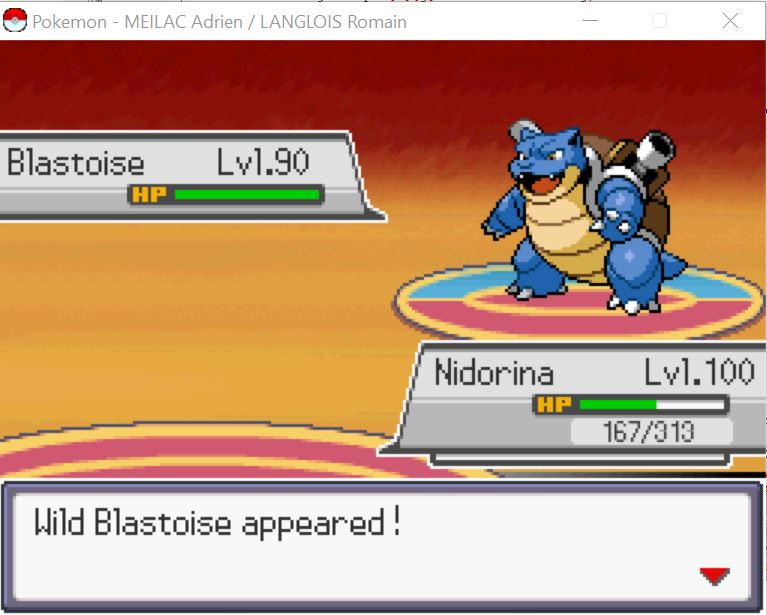
\includegraphics[scale = 0.6]{Graphiques/combat_start.jpg}
\end{minipage}
\begin{minipage}{0.49\textwidth}
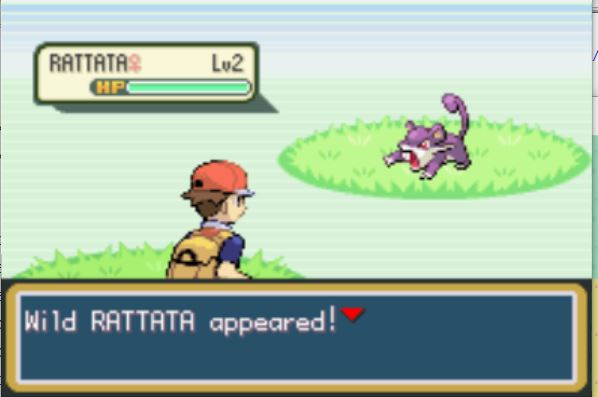
\includegraphics[scale = 0.84]{Graphiques/vrai_jeu_combat_start.jpg}
\end{minipage}
\caption{Début de combat}
\end{figure}

\begin{figure}[!h]
\begin{minipage}{0.49\textwidth}
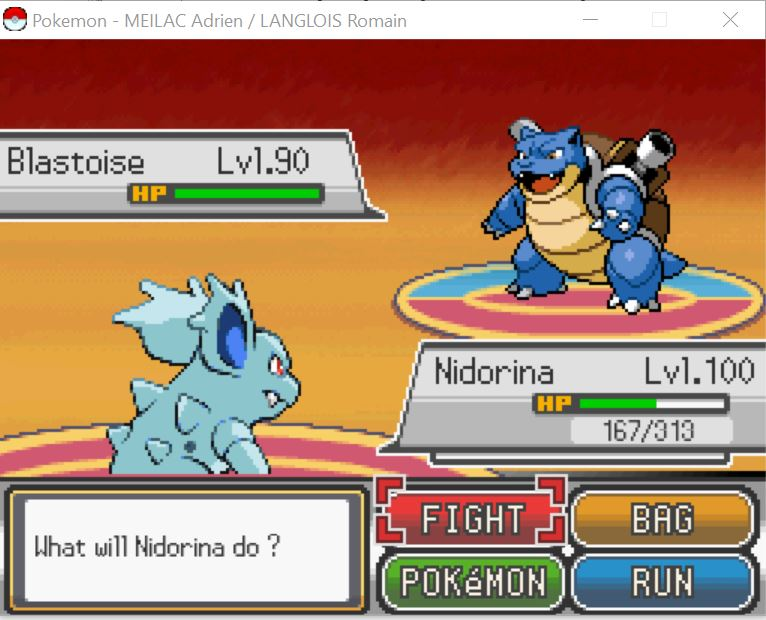
\includegraphics[scale = 0.6]{Graphiques/mainMenu.jpg}
\end{minipage}
\begin{minipage}{0.49\textwidth}
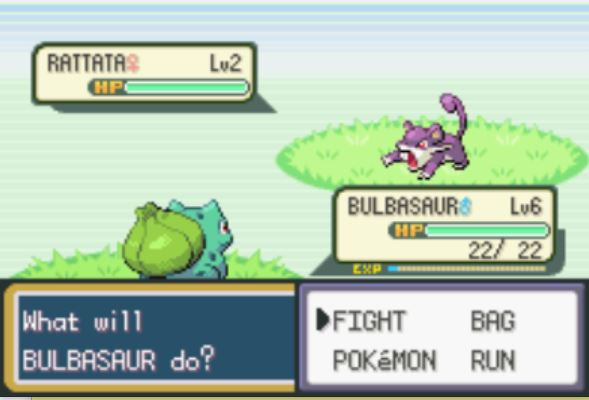
\includegraphics[scale = 0.84]{Graphiques/vrai_jeu_mainMenu.jpg}
\end{minipage}
\caption{Menu principal}
\end{figure}

\begin{figure}[!h]
\begin{minipage}{0.49\textwidth}
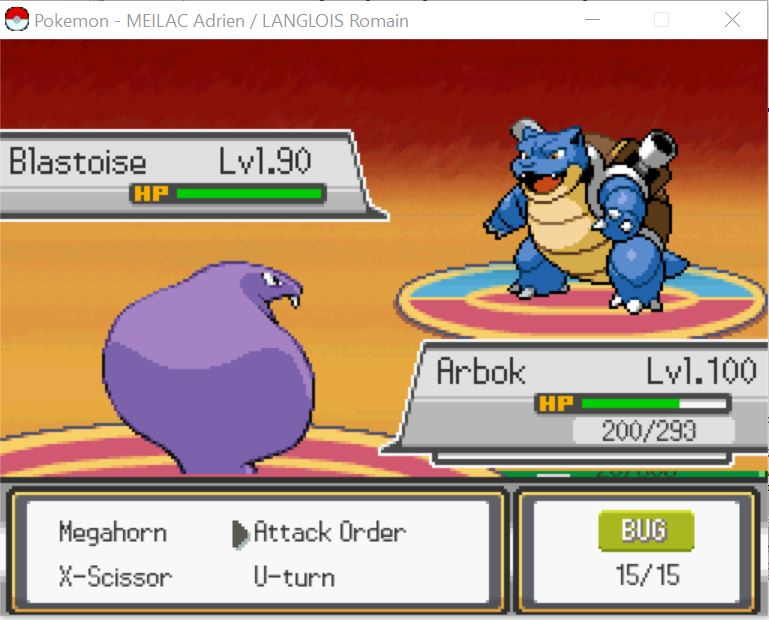
\includegraphics[scale = 0.6]{Graphiques/fightMenu.jpg}
\end{minipage}
\begin{minipage}{0.49\textwidth}
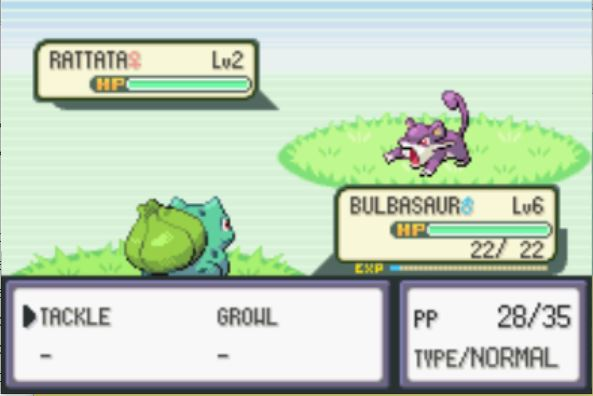
\includegraphics[scale = 0.84]{Graphiques/vrai_jeu_fightMenu.jpg}
\end{minipage}
\caption{Menu de combat}
\end{figure}

\begin{figure}[!h]
\begin{minipage}{0.49\textwidth}
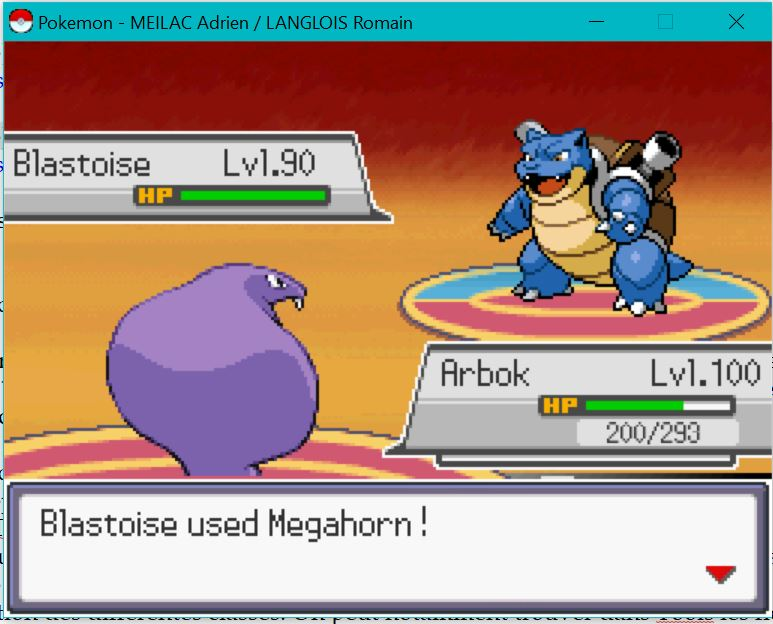
\includegraphics[scale = 0.6]{Graphiques/useMove.jpg}
\end{minipage}
\begin{minipage}{0.49\textwidth}
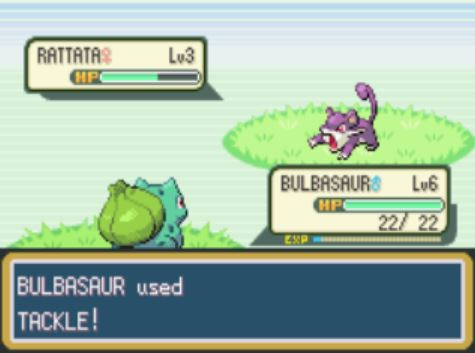
\includegraphics[scale = 0.84]{Graphiques/vrai_jeu_useMove.jpg}
\end{minipage}
\caption{Joueur sur la carte Pokémon}
\end{figure}

\begin{figure}[!h]
\begin{minipage}{0.49\textwidth}
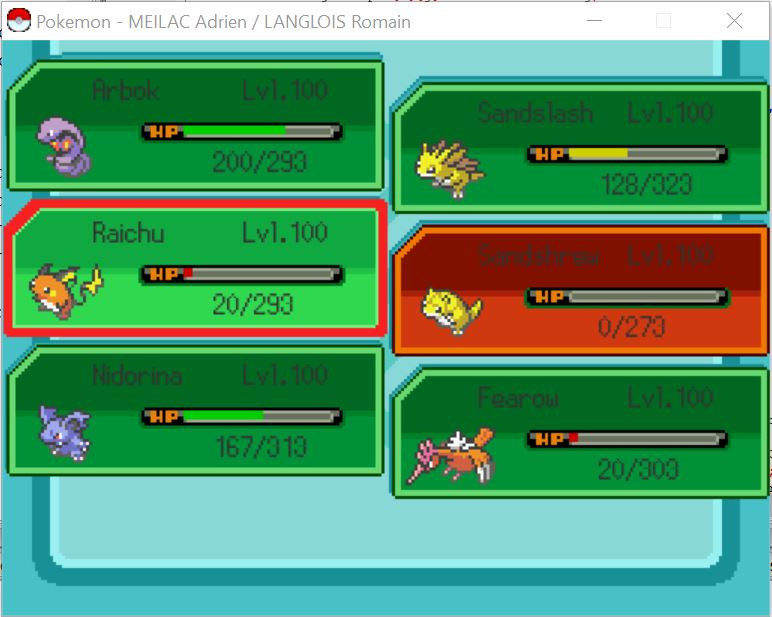
\includegraphics[scale = 0.6]{Graphiques/swapMenu.jpg}
\end{minipage}
\begin{minipage}{0.49\textwidth}
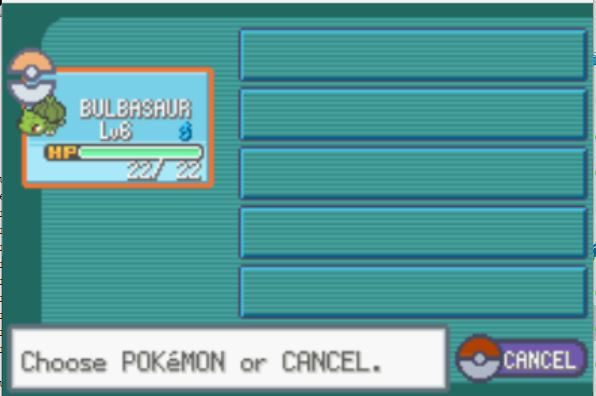
\includegraphics[scale = 0.84]{Graphiques/vrai_jeu_swapMenu.jpg}
\end{minipage}
\caption{Menu du dresseur}
\end{figure}

\begin{figure}[!h]
\begin{minipage}{0.49\textwidth}
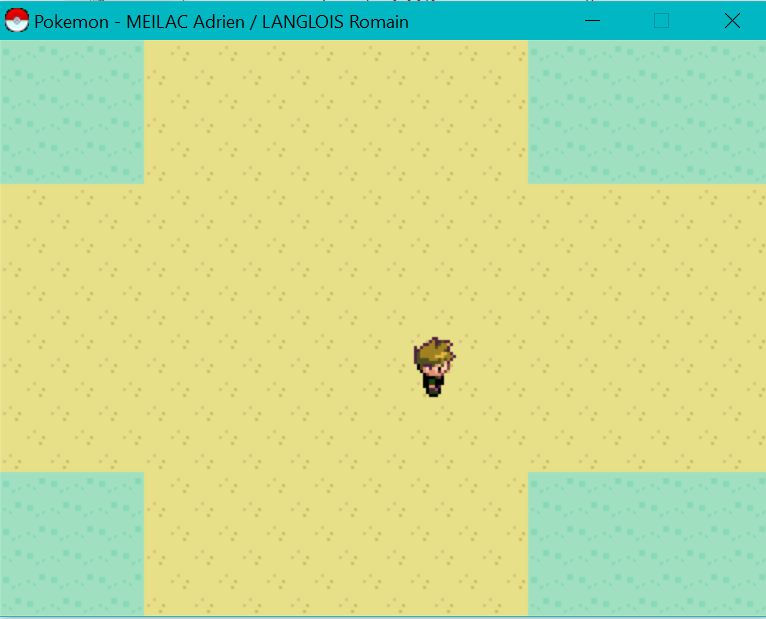
\includegraphics[scale = 0.6]{Graphiques/map.jpg}
\end{minipage}
\begin{minipage}{0.49\textwidth}
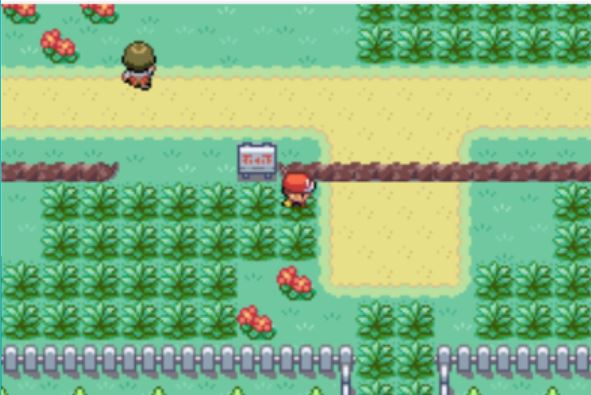
\includegraphics[scale = 0.84]{Graphiques/vrai_jeu_map.jpg}
\end{minipage}
\caption{Joueur sur la carte Pokémon}
\end{figure}

\newpage 

\section{Architecture du code}

D'après GitHub, notre code est composé de 35 fichier .cpp et de 23 fichier .h, et notre projet contient environ 11 000 lignes. Pour ne pas se perdre dans notre projet, nous avons donc essayé de hiérarchiser notre code. 

\subsection{Les différents répertoires}
Notre code est réparti dans répertoires suivants.
\subsubsection{Tools}
Tools contient tous les outils dont nous avons eu besoin lors de notre projet, qui ne sont pas directement relié au mécanisme de fonctionnement de notre jeu, mais qui permettre de simplifier la création des différentes classes. On peut notamment trouver dans Tools les fichiers (et leur header) suivants :
\begin{itemize}
\item \textbf{Table }: La totalité de nos fichiers sont des tableaux (avec comme délimiteurs '';''). C'est pourquoi il nous a paru essentiel de simplifier la lecture des fichiers en créant une classe qui les lirait. Cette classe est capable d'extraire une ligne, une colonne et surtout de donner un élément à partir de son nom de ligne et de son nom de colonne (surcharge de l'opérateur () car [] ne peut être surchargé qu'avec un argument). Afin de standardiser la saisie, nous avons décider que la lecture des tableaux donnerait uniquement des chaînes de caractères (et ne chercherait donc pas à donner des nombres). 
\item \textbf{VectorMethod} : Ce fichier contient des fonctions supplémentaires concernant les vecteurs. Notamment, un test vector\_in qui permet de dire si un élément est dans le vecteur, et une fonction qui permet de découper les chaînes de caractères. Cette dernière sert par exemple lors de la création des objets de type Table. 
\item \textbf{Conversion} contient une collection de fonctions permettant de convertir les objets d'un type à un autre. En effet, le compilateur MinGW fournit par notre IDE CodeBlocks ne nous laissait pas utiliser les fonction stoi, atoi stol ... qui permettent la conversion directe des types. Nous avons donc créé nos propres fonctions. Ces dernières sont généralement utilisées après la lecture des fichiers contenant des données pour convertir les std::string que la classe Table permet d'extraire (et donc de compenser le fait que Table ne soit composé que de std::string)

\item \textbf{Random} qui contient des fonctions plus simples pour faire appel à l'aléatoire. Nous avons eu des difficultés à utiliser la fonction std::uniform\_real\_distribution, c'est pourquoi nous avons créé une approximation de cette dernière à l'aide de rand()

\item  \textbf{StatSet} et \textbf{StatSetExt} sont des classes (la seconde héritant de la première) qui permettent de stocker les différentes statistiques de nos Pokémon. Lors de leur création, nous nous sommes aperçu que des arguments liés aux points de vie, d'attaque, de défense, d'attaque spéciale, de défense spéciale et de vitesse. Nous avons aussi mis dedans la formule permettant de calculer les statistiques d'un Pokémon. \\
Si on note
\begin{itemize}
\item \textbf{Niv}, le niveau d'un Pokémon, \\
\item \textbf{PV} sa vie maximum, \\
\item \textbf{Stat} la valeur de ses autres statistiques (Attaque Défense, Attaque Spéciale, Défense Spéciale, Vitesse) (cette valeur est celle qui est valable lorsque le Pokémon est soigné), \\
\item \textbf{IV} des paramètres pour chacune des statistiques (ces derniers varient entre 0 et 31, ils sont générés aléatoirement lors de la création d'un Pokémon, ils ne sont ni visibles ni modifiables),\\
\item \textbf{EV} des paramètres pour chacune des statistiques (ces derniers varient entre 0 et 255, ils valent 0 lors de la création d'un Pokémon et varient en fonction des combats effectués, ils ne sont pas visibles par l'utilisateur, mais ce dernier peut les modifier indirectement),\\
\item \textbf{Base} des paramètres pour chacune des statistiques traduisent l'influence de l'espèce sur un Pokémon,
\end{itemize}
alors les statistiques d'un Pokémon sont définies par :
\[
Stat = \Floor{\dfrac{2 * Base + IV + \Floor{\frac{EV}{4}} * Niv + 5}{100} * Nat}
\]
\[
PV =\Floor{\dfrac{2 * Base + IV + \Floor{\frac{EV}{4}} * Niv}{100}} + Niv + 10
\]
\end{itemize}

\subsubsection{Pokémon}
Pokémon est un répertoire qui contient l'architecture des classes que nous remplissons lorsque le programme est lancé. La plupart des classes ont un constructeur qui prend en paramètre un nom interne d'objet dont les caractéristiques sont définies dans un ou plusieurs fichiers. Le constructeur va alors utiliser la fonction Table pour lire la ligne du fichier qui l’intéresse et construire l'objet, ce qui simplifie énormément la déclaration des classes. Nous avons fait notre code de tel sorte que les arguments des uns sont les noms internes des autres ce qui permet de créer automatiquement les objets associés. 

Par ailleurs, la plupart des objets ont une structure qui n'est pas aléatoire et qui est totalement déterminé par le nom interne de l'objet, nous avons donc surchargé les operateurs == entre un objet et un std::string pour simplifier les déclarations d'égalité et rendre le code plus lisible (cela permet d'écrire par exemple if(type == ''FIRE'') ...)

Voici une description des différentes classes :

\begin{itemize}
\item \textbf{Type} contient la classe codant le Type des Pokémon ou des attaques. Les méthodes les plus importantes de cette classes sont effectiveness qui donne l'efficacité d'un Type sur un autre (par exemple, une attaque de type Eau sera très efficace contre un Pokémon de Type Feu), ainsi que getPathImage qui permet de donner l'image à afficher pour indiquer le Type d'un Pokémon.
\item \textbf{Move} contient la classe codant les attaques des Pokémon. Elle est lié au fichier ''Data/Move.txt'' qui contient énormément d'argument, parfois très complexes. Nous n'avons donc pas tout utilisé. Move contient des objets issus des classes Flag, Target et DamageCategory qui correspondent à des effets particuliers liés au attaques. Ces classes offrent une gamme de test booléen pour éviter d'avoir à gérer des notations abstraites. 
\item  \textbf{Species} contient les arguments liés à l'espèce d'un Pokémon. Nous avons décidé de sauvegarder les mouvements que peut apprendre un Pokémon (en moyenne, une centaine) sous forme de string pour ne pas utiliser inutilement de la mémoire étant donné que seul 4 sont utilisés (et sont donc converti en Move dans la classe fille Pokémon). 
\item  \textbf{Pokémon} contient principalement les fonctions qui permettent de faire varier les statistiques des Pokémon. On lui associe 2 Types, 4 Attaques, ainsi que deux structures de statistiques, l'une étant l'état normal, et l'autre l'état actuel (En effet, si un Pokémon est blessé, il n'a pas sa vie au maximum, cette information est stockée dans l'état actuel. Toutefois, si il est soigné, il revient à son état normal. Cet état normal peut aussi jouer dans le calcul des dégâts, d'où l’intérêt de le sauvegarder comme un argument). 
\end{itemize}

Les formules pour calculer les dégâts dans le vrai Pokémon sont assez compliqués :\\
Si on note :
\begin{itemize}
\item Att la statistique d'attaque si le Move est physique, l'attaque spéciale si l'attaque est spéciale
\item Def la statistique de défense si le Move est physique, l'attaque spéciale si l'attaque est spéciale
\item Power le pouvoir de base (statistique lié à Move)
\item Weather l'effet du temps
\item Badge l'effet lié aux badges de l'utilisateur
\item Critical l'effet bonus aléatoire 
\item random , un nombre entre 0.85 et 1
\item STAB, l'effet bonus si le Pokémon est du même type que son attaque
\item Type, l'effet du type de l'attaque sur le Pokémon
\end{itemize}
alors 
\[
Damage = \Floor{\left(\dfrac{\left(\dfrac{2 * Niv}{5} + 2\right) * Power * \dfrac{Att}{Def}}{50} + 2 \right) * Modifier}
\]
avec
\[
Move = Targets * Weather * Badge * Critical * random * STAB * Type * Other
\]
nous avons donc choisi de faire des simplifications car il nous était impossible de coder tout ces effets qui ont été rajouté dans les différentes versions du jeu depuis plusieurs décennies.


\subsubsection{Battle}
Battle est un répertoire qui contient les fonctions liées aux fonctionnements des combats. Nous avons choisi de séparer les effets visuels (stockés dans Graphics) du système du jeu en lui même afin de créer des classes de combats qu'on lance via la méthode start et qui sont indépendantes. Nous avons préféré éviter d'avoir des codes trop long avec des fenêtres graphiques car le mécanisme interne des combats est complexe et cela aurait été une source d'erreur.

Dans le répertoire Battle, il y a :
\begin{itemize}
\item Player : qui contient les informations 

\end{itemize}


\end{document}

%\begin{lstlisting}
%int main()
%{
%	int a = 3;
%	std::string mot = ''je suis'';
%	return 0;
%}
%\end{lstlisting}